\documentclass[bibliography=totocnumbered]{scrartcl}
\usepackage{imakeidx}
\usepackage{ragged2e}
\usepackage{setspace} % Um den Zeilenabstand zu ändern.
\usepackage{gensymb}
%\usepackage{authblk}
% \usepackage{minitoc} % for the chpaters
\usepackage{wasysym}
%\usepackage{SI}
\usepackage{array} % Verwendung von Matrizen
\usepackage{booktabs} % Schöne Tabellen beziehungsweise sie sehen damit professioneller aus.
\usepackage{tabulary} % Ähnlich wie tabularx, ermöglicht aber das ändern der Ausrichtung der Spalten.
\usepackage{tabularx} % Tabellen mit automatischen Zeilenumbruch.
\usepackage{enumitem}
\usepackage{physics}
\usepackage[T1]{fontenc}% fontec und inputenc ermöglichen
\usepackage{graphicx}%Für Grafiken
\usepackage{rotating} % lässt Grafiken rotieren
\usepackage{mathtools}% mathematische Werkzeuge
\usepackage{amsmath}% Mathetools
\usepackage{amsfonts}% Mathetools
\usepackage{amssymb}% Symbole wie Natürliche Zahlen
\usepackage{geometry}
%\usepackage{bibtex} 
\usepackage{tablefootnote}% Fußnoten in Tabellen
\usepackage{float}% für eingebundene Bilder
\usepackage{fancyhdr} % Seiten schöner gestalten, insbesondere Kopf- und Fußzeile
\usepackage{ulem} 
\usepackage{dcolumn}% Align table columns on decimal point
\usepackage{bm}% bold math
\usepackage[ngerman]{babel} % Worttrennung nach der neuen Rechtschreibung und deutsche Bezeichnungen. babelfunktion wird wegen Literatur gebraucht.
\usepackage{subfloat} % Was macht diese Packet?
\usepackage{caption} % Unter-/Überschriften für Bilder, Grafiken und Tabellen
\usepackage{subcaption}
\usepackage{txfonts}
\usepackage{titling}% Titel
\usepackage[style=alphabetic]{biblatex} %biblatex mit alphabetic laden. alphbetic=Zitationsstil
\usepackage{bookmark}
\usepackage[printonlyused]{acronym}
\usepackage{amsthm}
\usepackage{pdfpages}
\usepackage{tikz}
\usepackage[siunitx,americanvoltages, europeanresistors,americancurrents]{circuitikz}
\usepackage{listings}
\usepackage{abstract}
\usepackage[per-mode = fraction]{siunitx}
\usepackage{hyperref}
\newcommand{\R}{\mathbb{R}} % reelle Zahlen
\newcommand{\N}{\mathbb{N}} % natürliche Zahlen
\newcommand{\C}{\mathbb{C}} % komplexe Zahlen
\newcommand{\Q}{\mathbb{Q}} % rationale Zahlen
\newcommand{\Z}{\mathbb{Z}} % ganze Zahlen
\newcommand{\F}{\mathbf{F}} % Kraft
\newcommand{\E}{\mathbf{E}} % Energie
\newcommand{\V}{\mathbf{v}} % Geschwindigkeit
\newcommand{\B}{\mathbf{B}} % magnetischer Fluss
\newcommand{\J}{\mathbf{j}} % Stromdichte ?
\newcommand{\D}{\mathbf{D}} % elektrische Induktion
\newcommand{\HH}{\mathbf{H}} % magnetische Feldstärke
\newcommand{\M}{\mathbf{M}} % Magnetisierung
\newcommand{\p}{\mathbf{P}}
\newcommand{\rr}{\mathbf{r}}
\newcommand{\vp}{\varphi}
\newcommand{\ve}{\varepsilon}
\newcommand{\vcc}[1]{\left(\begin{matrix}#1\end{matrix}  \right)}
\newcommand{\m}[1]{\left\lbrace #1\right\rbrace}
\newcommand{\los}{\noindent\textbf{Lösung}:}
\newcommand{\rang}[2]{\text{Rang}(#1)=#2}
\newcommand{\vpe}{\frac{1}{4\pi\ve_0}}
\newcommand{\qvpe}{\frac{q}{4\pi\ve_0}}
\newcommand{\geg}{\ac{geg.}}
\newcommand{\ges}{\ac{ges.}}

\newcommand{\kommando}[1]{$\backslash$\textit{#1}}
\newcommand{\com}[1]{$\backslash$\textit{#1}$\left\lbrace\ldots\right\rbrace$}
\newcommand{\Com}[2]{$\backslash$\textit{#1}$\left\lbrace #2\right\rbrace$}
\newcommand{\NeuKommando}[2]{$\backslash \textit{#1} \left\lbrace \backslash \textit{#2}\right\rbrace$}
\newcommand{\latex}{\LaTeX $\;$}


% si unitx
\DeclareSIUnit\litre{l}

\hypersetup{
	colorlinks=true,
	linkcolor=blue,
	filecolor=magenta,      
	urlcolor=cyan,
	citecolor=lime!50!black,
	filecolor=red
}
%\addbibresource{} %Bibliographiedateien laden
\addbibresource{bib.bib}

\geometry{a4paper, left=25mm, right=25mm, top=30mm, bottom=30mm}
\lhead{\thedate}
\rhead{GPR}
\lhead{\thetitle}
\pagestyle{fancy}

\usetikzlibrary{patterns}
\usetikzlibrary{3d}
\makeindex[title=Stichwortverzeichnis,intoc
,options= -s Index-Formatierung.ist
]
\author{Ben J. F.}
\allowdisplaybreaks

\lstset
{ %Formatting for code in appendix
    basicstyle=\footnotesize,
    numbers=left,
    stepnumber=1,
    showstringspaces=false,
    tabsize=2,
    breaklines=true,
    breakatwhitespace=false,
}


\title{M3 \\ Elastizität und Torsion}
\date{30.06.2021}
\begin{document}
	\newgeometry{left=14mm, right=13.5mm, top=60mm, bottom=30mm}
	\begin{titlepage}
		\begin{center}
			{\huge{Grundpraktikum}}\\\vspace*{15mm}
			{\huge{\textbf{\thetitle}}}\\\vspace*{20mm}
			{\theauthor}\\\vspace*{10mm}
			{\thedate}\\\vspace*{20mm}
			
			\vspace{1.5cm}
			\begin{abstract}
				In diesem Versuch soll das Elastizitätsmodul $ E $ mittels Längenänderung $ \Delta l $ berechnet werden. Weiterhin soll das Torsionsmodul $ G $ mittels Periodendauer $ T $ bestimmt werden. Aus dem Elastitäts- und Torsionsmodul wird zum Schluss die Poissonzahl errechnet. \\
				Die Ergebnisse lauten wie folgt:
				
			\begin{table}[ht!]
				\centering	
				\begin{tabular}{|c|c|c|}
					\hline
					 &                      Platz 1 &          Platz 3 \\
					\hline
					Elastizitätsmodul $ E $ $ \left[\text{N m}^{-2} \right]$ &            $ (8.58\pm0.06)10^{10}  $&  $ (9.3\pm 0.9)10^{10} $\\
					Torsionsmodul $ G $ $ \left[\text{N m}^{-2} \right]$ &  $ (3.6584502\pm0.0000005)10^{10} $&  $ (3.9\pm0.5)10^{10} $ \\
					Poissonzal $ \mu $                             &                $ 0.175\pm 0.011 $ &      $ 0.20\pm0.08 $ \\
					\hline
				\end{tabular}
				
			\end{table}
				
			\end{abstract}
			
			
		\end{center}
	\end{titlepage}
	\makeatother
	\restoregeometry
	\newpage
	
	\tableofcontents
	
	
	\listoffigures 
	\listoftables
	\newpage
	
	
	\section{Motivation und \\theoretische Vorbetrachtungen}
	Motivation dieses Experimentes war die Materialkonstanten der Elastizität zu berechnen, hier speziell Elastizitätsmodul E, Torsionsmodul G und die Poissonsche Zahl $ \mu $.\\\\
	Um diese zu berechnen benutzen wir die Querkontraktion und Dehnung um das Elastizitätsmodul zu bestimmen und das Torsionsmodul aus der Drehschwingung zu bestimmen.\\\\
	Für die Berechnung des Elastizitätsmoduls gilt für die angreifende Gravitationskraft:
\begin{equation}\label{eq: Delta l}
	\Delta l=\dfrac{1}{E}\dfrac{l_{0}}{A}gm
\end{equation}
Wobei die Längenänderung entspricht, $ A $ die Queschnittsfläche des Körpers, $ l_{0} $ die Länge des Objektes (hier ein Messing draht), $ g $ die Erdbeschleunigung ($ g=(9.8130\pm 0.0001 )$ms$ ^{-2} $\smartcite{Muller.b}) und $ m $ die Masse.\\\\
Für die Drehschwingung mit einem zusätzlichen Trägheitsmoment einer Drehscheibe gilt:
	\begin{align}\label{eq: Torsionsmodul}
		G=\dfrac{4\pi l_{0}}{R^{4}}\dfrac{mr^{2}}{T_{s}^{2}-T_{v}^{2}}
	\end{align}
	Mit $ m $ der Masse der Drehscheibe, $ t $ dem Radius der Drehscheibe, $ R $ dem Radius der schwingungsfähigen Anordnung, $ T_{s} $ die Periodendauer mit der Scheibe, $ T_{v} $ die Perioden ohne die Scheibe.\\
	Allgemein gilt die Beziehung für die Possion Zahl, Torsionsmodul und dem Elastizitätsmodul.
	
	\begin{equation}\label{eq: Poisson Zahl}
		\mu= \dfrac{E}{2G}-1
	\end{equation}
Die Herleitung und tieferführende Erläuterungen finden Sie im Versuchsskript\smartcite{Muller.e}.
	
	\section{Versuchsbeschreibung}
	\subsection{Bestimmung des Elastizitätsmoduls}
	Hier wird mit Hilfe von Massen ein Messingdraht durch die Gravitationskraft gedehnt und die Längenänderung gemessen, mittels einer Millimeterschraube und Libelle. Dies findet in 50g Schritten statt von $ 50 $g bis $ 800 $g dabei wird die gemessene Länge des unbelasteten Zustandes abgezogen von dem der Belasteten.
	
	\subsection{Bestimmung des Torsionsmoduls}
	Hier wird ein 50g Stück an die Schraube angebracht und dann für 6 Perioden 6 mal die Periodenzeit gemessen der Drehung.\\
	Dieses wiederholt man mit einer Drehscheibe ebenso.
	
	
	\newpage
	\section{Berechnung des Elastizitätsmoduls}
	Die Datensätze werden mittels lineare Regression gemäß dem Material \cite{MullerPG.2007b} der Form, $ y=mx $, graphisch ausgewertet.\\
	Daraus ergibt sich die lineare Regression.
	\begin{equation}\label{eq: lin Regr}
		\Delta l=\dfrac{1}{E}\dfrac{l_{0}}{A}gm=am
	\end{equation}
	Mit $ a $, dem Anstieg.
	
	\begin{figure}[!ht]
		\centering								 
		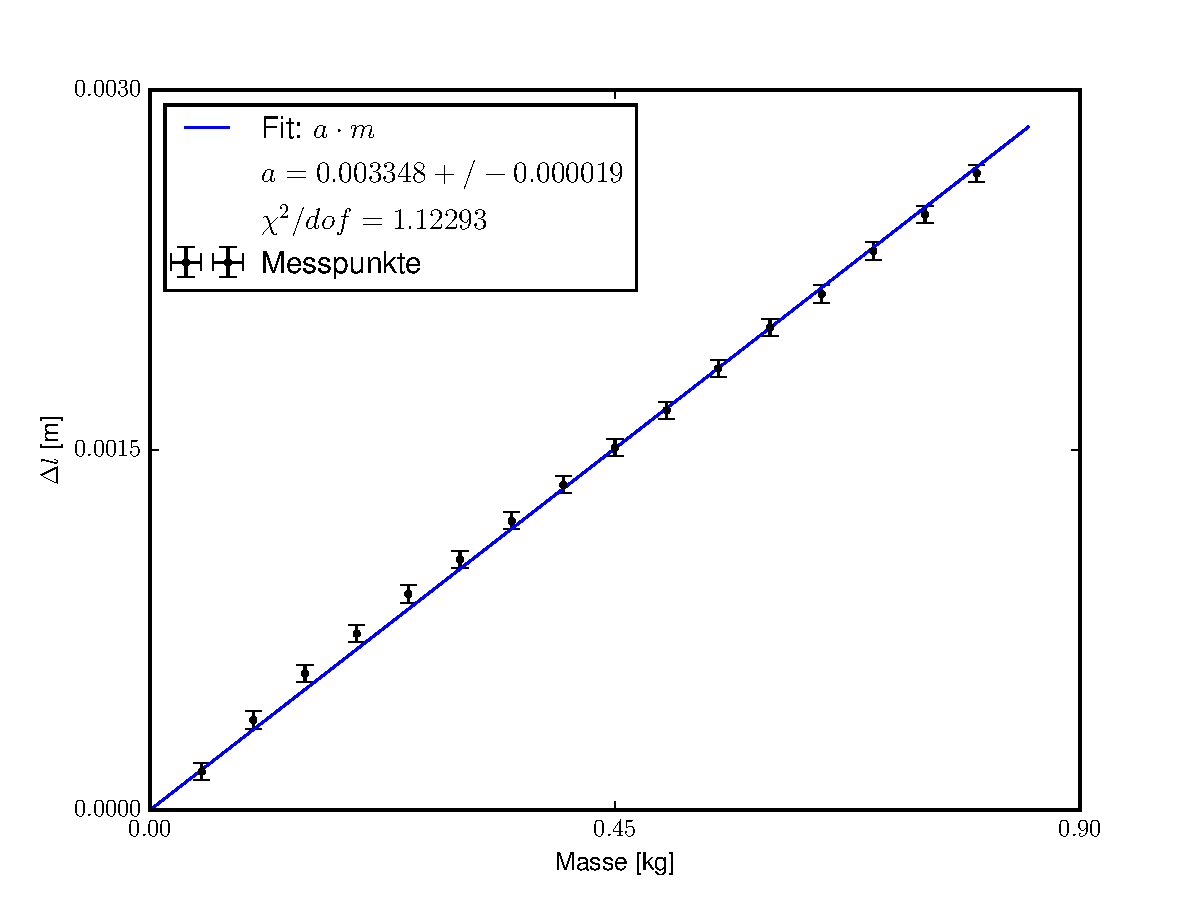
\includegraphics[width=250pt]{fotos/gpr1/M3_B_MR1.pdf}			 
		\caption[Messreihe 1, Platz 3]{Längendifferenz in Abhängigkeit zur Masse, Aufhängung von Massestücken}							 
		\label{Abb: M1, P3}							 
	\end{figure}
	
	\begin{figure}[!ht]
		\centering								 
		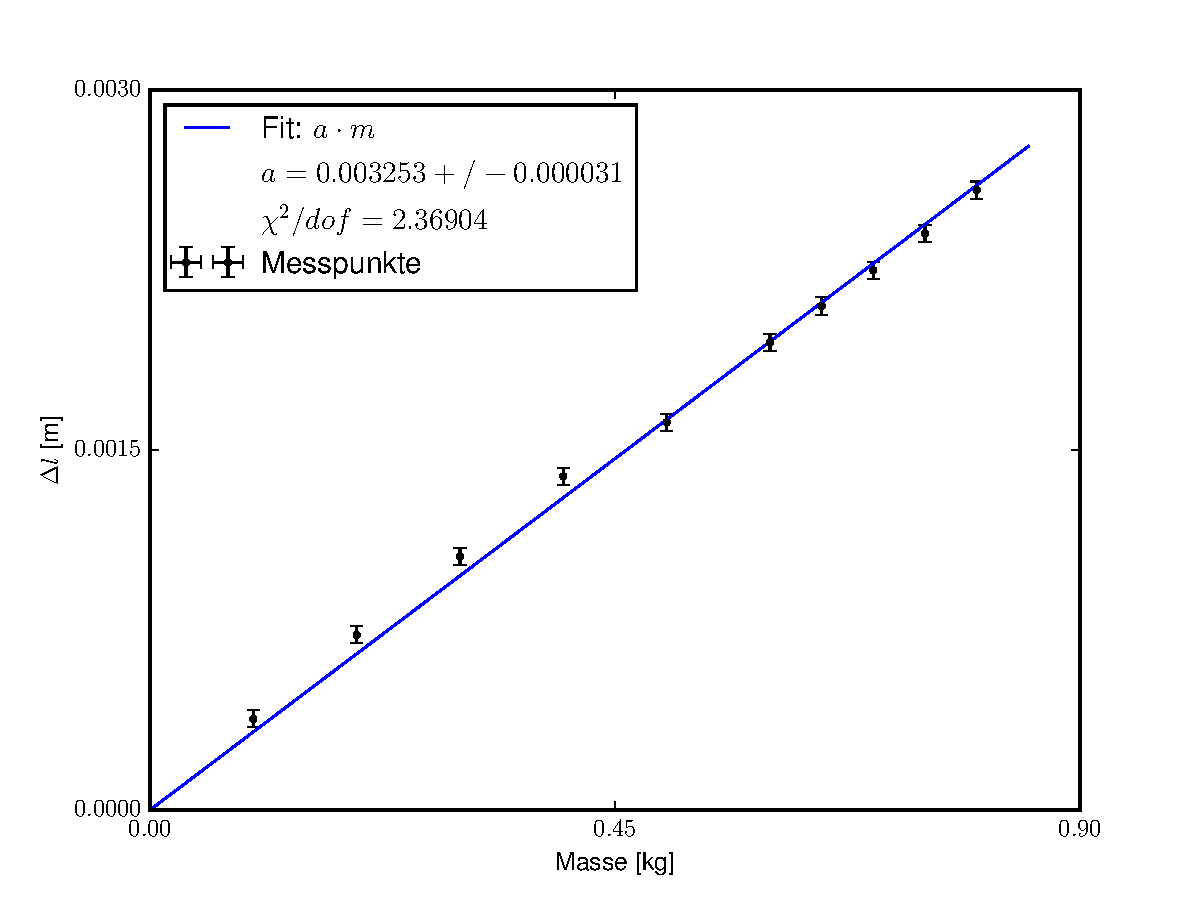
\includegraphics[width=250pt]{fotos/gpr1/M3_B_MR2.pdf}			 
		\caption[Messreihe 2, Platz 3]{Längendifferenz in Abhängigkeit zur Masse, Abhängung von Massestücken}							 
		\label{Abb: M2, P3}							 
	\end{figure}
	
	\begin{figure}[!ht]
		\centering								 
		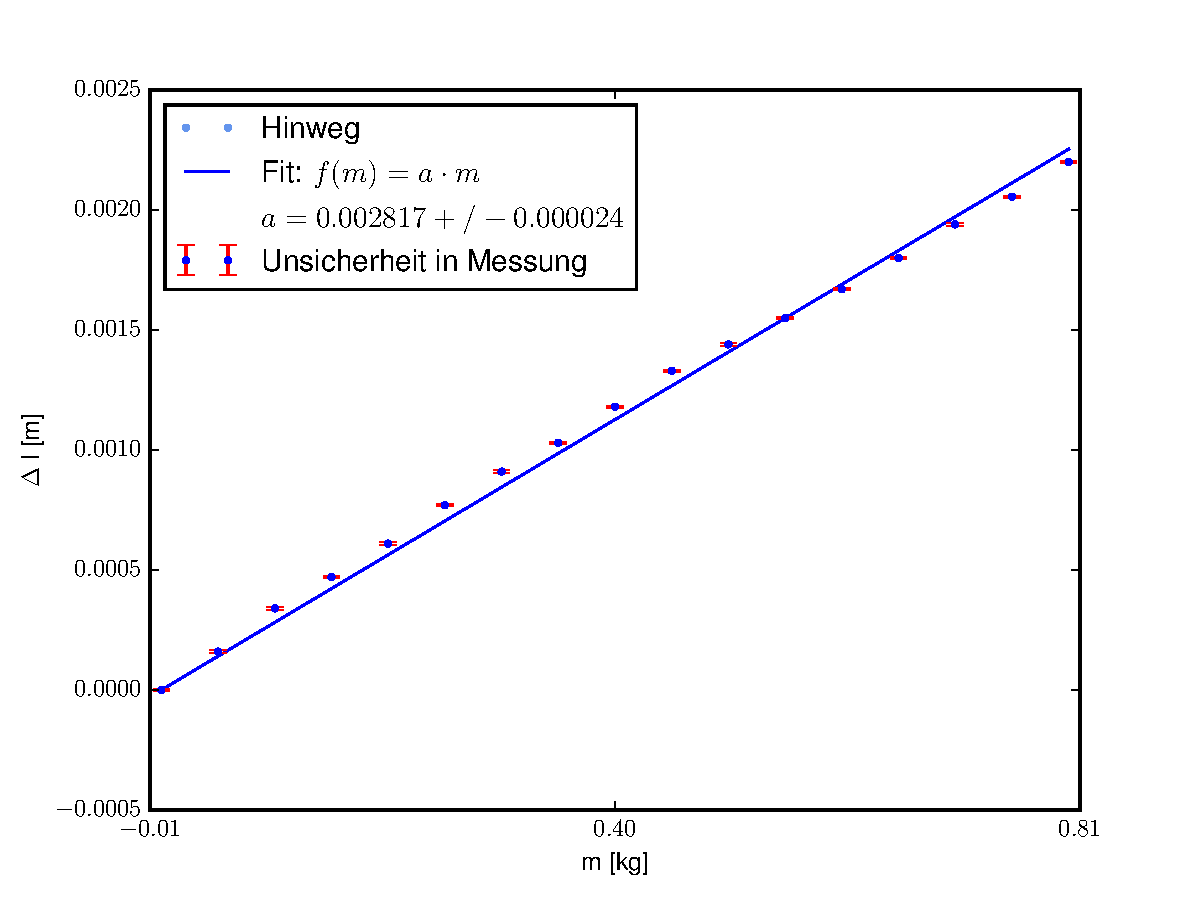
\includegraphics[width=250pt]{fotos/gpr1/M3_MR1_S.pdf}			 
		\caption[Messreihe 1, Platz 1]{Längendifferenz in Abhängigkeit zur Masse, Aufhängung von Massestücken}							 
		\label{Abb: M1, P1}							 
	\end{figure}

\begin{figure}[!ht]
	\centering								 
	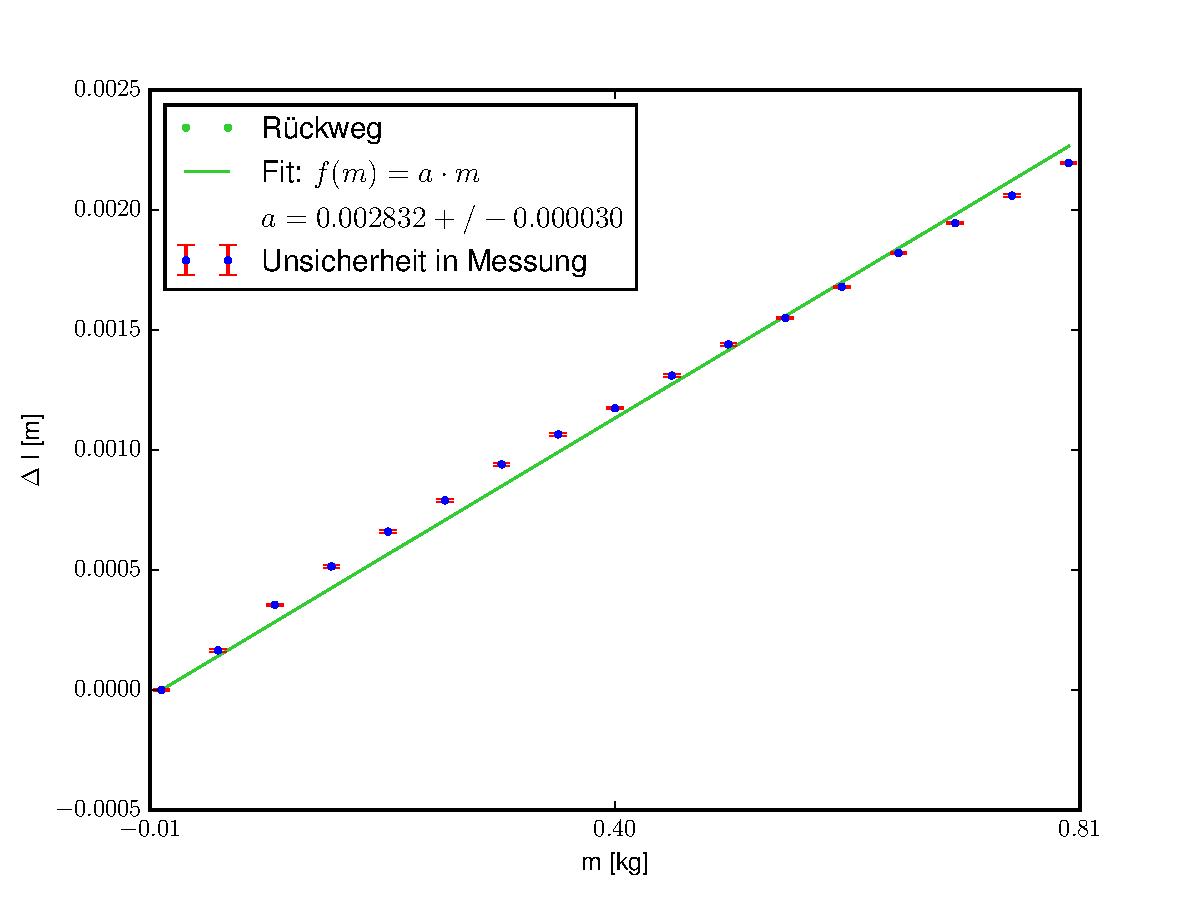
\includegraphics[width=250pt]{fotos/gpr1/M3_MR2_S.pdf}			 
	\caption[Messreihe 2, Platz 1]{Längendifferenz in Abhängigkeit zur Masse, Abhängung von Massestücken}							 
	\label{Abb: M2, P1}							 
\end{figure}
	
	\newpage
	
	Dabei hat die Längenänderung die Unsicherheit des Ablesens der Skala mit 0.005mm, aber ebenso den Fehler durch die Libelle von 0.02mm. Beides wird noch mit Wurzel 2 aufgrund der Differenz multipliziert.\smartcite{MullerPG.2007b}
	Hierbei ist der x-Achsen Fehler zu klein, um aufgenommen zu werden
	Der lineare Zusammenhang scheint so mit bestätigt.
	\\\\
	Daraus ergeben sich die Parameter:
	\begin{table}[ht!]
		\centering
		\caption{Regressionsanstiege}
		\begin{tabular}{|c|c|c|}
			\hline
			Steigung & Platz 1 & Platz 3 \\
			\hline
			Massenanstieg $ \left[\text{m}^{2}\text{ N}^{-1}\text{ s}^{-2}\right] $& $ (28.17\pm 0.21)10^{-4} $ & $ (33.48 \pm 0.19)10^{-4} $ \\
			\hline
			Massenabstieg $ \left[\text{m}^{2}\text{ N}^{-1}\text{ s}^{-2}\right] $& $ (28.3 \pm0.3 )10^{-4} $ &$ (32.5 \pm 0.3)10^{-4} $  \\
			\hline
		\end{tabular}
		\label{tab: Regr. anstiege}
	\end{table}
	
	\newpage
	
	\subsection{Berechnung von E}
	Aus der Steigung ergibt sich nun der E-Wert von\\
	\begin{equation}\label{eq: E Modul}
		E= \dfrac{l_{0}}{a \cdot A}g
	\end{equation}
	Damit ergeben sich folgende E-Werte:
	\begin{table}[ht!]
		\centering 
		\caption{Ergebnisse für das E-Modul}
		\begin{tabular}{|c|c|c|}
			\hline
			& Platz 1 & Platz 2 \\
			\hline
			Messreihe 1  $ \left[\text{N m}^{-2} \right]$&$ (8.60\pm0.08)10^{10} $  &$(9.2\pm0.6)10^{10}  $  \\
			\hline
			Messreihe 2 $ \left[\text{N m}^{-2} \right]$&$(8.55\pm0.10)10^{10}  $  & $ (9.5\pm0.6)10^{10} $ \\
			\hline
			\hline
			gewichtetes Mittel  $ \left[\text{N m}^{-2} \right]$&  $ (8.58\pm0.06)10^{10}  $&  $ (9.3\pm 0.4)10^{10} $ \\
			\hline
		\end{tabular}
		\label{tab: E Werte}
	\end{table}
	\section{Berechnung des Torsionsmoduls}
	Für den Versuch wurde die Zeit für 6 Perioden sechsmal gemessen mit der Belastungsmasse 50g. Danach wurden die Zeiten gemittelt.\\
	Aus der Gleichung (\ref{eq: Torsionsmodul}) ergeben sich folgende Werte des Torsionsmoduls:
	
	\begin{table}[ht!]
		\centering
		\caption{Torsionsmodul Ergebnisse}
		\begin{tabular}{|c|c|c|}
			\hline
			& Platz 1 & Platz 3 \\
			\hline
			Torsionmodul $ \left[\text{N m}^{-2} \right]$&  $ (3.66\pm0.03)10^{10} $&  $ (3.9\pm0.5)10^{10} $  \\
			\hline
		\end{tabular}
		\label{tab: ergebnisse Torsionsmodul}
	\end{table}
	
	Die Fehler wurden mittels Gauß'scher Fehlerfortpflanzung berechnet.
	
	

	
	
	
	
	
	
	
	
	
	\section{Berechnung der Poisson Zahl}
	
	Da $ E $ und $ G $ bekannt sind, kann man nun mit der Formel (\ref{eq: Poisson Zahl}) die Poissionzahl bestimmen.\\
	Die Ergebnisse lauten somit:
	
	\begin{table}[ht!]
		\centering
		\caption{Ergebnisse zur Poisson Zahl}
		\begin{tabular}{|c|c|c|}
			\hline
			& Platz 1 & Platz 3 \\
			\hline
			Poisson Zahl &$ 0.175\pm 0.011 $ &      $ 0.20\pm0.08 $  \\
			\hline
		\end{tabular}
		\label{tab: ergebnisse Poisson zahl}
	\end{table}
	Die Fehler wurden mittels Gauß'scher Fehlerfortpflanzung berechnet.
	
	\section{Chi Quadrat}\label{sect: chi quadrat}
	Zur Einschätzung der Genauigkeit der Messung kann man $ \chi^{2} $ verwenden. Die Formeln dazu findet man im allgeimeinen Praktikumgsskript\smartcite{MullerPG.2007b}.
	\begin{table}[ht!]
		\centering
		\caption{$ \chi^{2} $ Ergebnisse}
		\begin{tabular}{|c|c|c|}
			\hline
			& Platz 1 & Platz 3 \\
			\hline
			Massen aufhängend & 1.865 & 1.1 \\
			\hline
			Massen abhängend & 3.08 & 2.4 \\
			\hline
		\end{tabular}
		\label{tab: chi quadrat}
	\end{table}
	Beim $ \chi^{2} $ wird für eine reelle Messung innerhalb des Praktikums ein Wert von 1 erwartet.
	Somit liegen die aufhängenden Messreihen beide gut im Erwartungswert zu liegen, was bedeutet, dass die Messung erfolgreich war und Fehler gut genug abgeschätzt wurden.\\\\
	Bei der abhängenen Messreihe ergab sich ein $ \chi^{2} $ von 3 und 2, was unteranderem daran lag, dass die Wasserwaage sich nicht ausrichten wollte und die Luftblase oft gewandert war, womit eine genaue Messung schwierig war. Außerdem könnte dadurch dass nicht 50g Stücke genommen wurden, sondern 100 g und ein 50 g Schritt beim wieder aufhängen des 50 g Stückes ein Fehler unterlaufen sein, indem man den Draht runter gezogen hat.
	
	\section{Fehlereinschätzung}
	\subsection{Fehlerfreie Werte}
	Für Platz 1 wurde angenommen, dass die Gravitationskonstante fehlerfrei ist, die sind jedoch ebenso fehlerbehaftet. Jedoch sind die Fehler so klein, dass diese bei der Rundung vernachlässigt worden wären, somit vernachlässigt werden können.\\
	Für Platz 3 wurde dies nicht angenommen und der entsprechende Wert wurde aus dem Versuchskript\smartcite{Muller.b} für die Federkonstante entnommen.
	
	\subsection{Zeitmessung}
	Bei der Messung der Periodendauer wurde eine digitale Stoppuhr genutzt. Dort muss man neben dem Gerätefehler noch zweimal die Reaktionszeit von ca. 0.25s als Unsicherheit nehmen. Die sind bei den kleinen Zeiten, die man gemessen hatte so groß, dass kaum der Gerätefehler beachtet werden musste.
	
	\subsection{Reibung und Annahme eines harmonischen Oszillators}
	Wir nehmen an, dass bei der Bestimmung der Periodendauer für das Torsionsmodul es sich um eine harmonische Schwingung handelt, sprich der Dämpfungsfreiheit der Schwingung. Dies jedoch trifft kaum zu, da es wie im jeden realen Versuch Reibung gibt.
	
	\subsection{Längenmessung}
	Fehler der Längenmessungen:\\
	- Skala (Libelle)\smartcite{Wikipedia.2019}\\
	- Millimeterschraube\\
	Die Justierung der Libelle war, wie in Kapitel \ref{sect: chi quadrat} erwähnt, sehr schwer, da sich die Luftblase oft bewegte, was die Messung erschwerte.\\
	Dies hat auch die Unsicherheit stark beeinflusst da bevor man die Unsicherheit von 0.02mm angenommen hatte, dass sich sonst ein Chi Quadrat von ca. 30 für die Messung ergab.
	\newpage
	\section{Schlussfolgerung}
	Das Experiment scheint ein Erfolg zu sein, da alle Werte sinnvolle Ergebnisse liefern (wie die Poission Zahl zwischen 0 und 0.5 liegt, wie im Versuchskript\smartcite{Muller.e} beschrieben) und die lineare Regression ebenso bestätigt wurde.\\\\
	Anzumerken wäre, dass es sich nicht nur um ab und aufhängen von Gewichten handelte, was der Aufgabenstellung etwas widerspricht. Dem entsprechend wäre es besser nur 50g Stücke zu verwenden.\\\\
	Die Messung der Länge mit der fehleranfälligen Libelle kann nicht ersetzt werden, da nur die Millimeterschraube die kleinen Längenänderungen messen kann. Da würde ich nur empfehlen etwas mehr zu üben, um ein besseres Gefühl zu bekommen.\\\\
	Ebenso könnte versuchen zu überprüfen, ob die Temperatur wirklich die Elastizität verändern würde, indem man zum Beispiel einen Heizstrahler verwenden könnte.\\\\
	Alles in allen ist das Experiment gelungen und die Ergebnisse zufriedenstellend.
	
	\appendix
	\newpage
	\printbibliography[title={Quellenverzeichnis}]
	
	
\end{document}